\documentclass[polish,a4paper,11pt]{mwart}

\usepackage[polish, english]{babel}
\usepackage[utf8]{inputenc}
\usepackage{polski}
\usepackage[T1]{fontenc}
\usepackage{lmodern}  % zestaw fontów
\usepackage{indentfirst}
\frenchspacing

\usepackage{enumerate}
\usepackage{graphicx}
\usepackage{float}
\usepackage{makecell}
\usepackage{siunitx}
\sisetup{output-decimal-marker = {,}}
\usepackage{icomma}
\let\lll\undefined
\usepackage{amsmath, amssymb, amsfonts}
\usepackage{mathtools}
\usepackage{import}		% wklejanie pdf_tex
\usepackage{xcolor}		% kolory
\usepackage{multirow}
\usepackage{microtype}
\usepackage{tabularx}
\usepackage{pgfplots}

\usepackage[%			% bibliografia
style=numeric,
sorting=none,
language=autobib,
autolang=other,
backend=biber,
]{biblatex}

\usepackage{csquotes}
\DeclareQuoteAlias{croatian}{polish}

\addbibresource{bibliografia.bib}

\usepackage{placeins}	% poprawia float

\let\Oldsection\section
\renewcommand{\section}{\FloatBarrier\Oldsection}

\let\Oldsubsection\subsection
\renewcommand{\subsection}{\FloatBarrier\Oldsubsection}

\let\Oldsubsubsection\subsubsection
\renewcommand{\subsubsection}{\FloatBarrier\Oldsubsubsection}

\AtBeginDocument{
  \renewcommand{\tablename}{Tab.}
  \renewcommand{\figurename}{Rys.}
}

\setlength{\emergencystretch}{3em}

\DeclareSIUnit\decibelV{dBV}

\date{\today}
\author{Zuzanna Kusal, Szymon Mikulicz, Marcel Piszak, Anna Warowny}
\title{Sprawozdanie z projektu redukcji drgań płyty}

\begin{document}

\maketitle

\section{Cel}

Celem projektu było zaprojektowanie, zamodelowanie i zbudowanie podzespołu
układu do redukcji drgań płyty kwadratowej, jednostronnie utwierdzonej,
pobudzonej do drgań w częstotliwościach własnych, a następnie przeprowadzenie
redukcji dla 5 częstotliwości własnych drgań wywołanych wzbudnikiem, z
wykorzystaniem 1 lub 2 aktuatorów względem 1 lub 2 czujników (9 konfiguracji
dla każdej częstotliwości).

\section{Identyfikacja częstotliwości własnych} \label{ident}

Przed przystąpieniem do redukcji drgań zmierzono częstotliwości drgań własnych
zmontowanego układu. Posłużono się oprogramowaniem napisanym w środowisku
LabVIEW\texttrademark, które podawało sygnał wymuszenia pod postacią sinusa
przestrajanego na wzbudnik i rejestrowało sygnały pochodzące z czujników. Na
rysunku \ref{fig:mody} przedstawiono uzyskany rozkład amplitud.

\begin{figure}[!tbh]
  \input{plots/mody.pgf}
  \caption{Rozkład amplitud dla czujników}
  \label{fig:mody}
\end{figure}

W programie Salome-Meca zamodelowano płytę kwadratową, jednostronnie
utwierdzoną, o wymiarach \SI{220 x 220 x 1}{\milli\meter}. Przeprowadzono analizę
modalną i uzyskano postacie drgań własnych  oraz odpowiadające im
częstotliwości w zakresie do \SI{1.5}{\kilo\hertz}.

Wartości teoretyczne częstotliwości obliczono ze wzoru:
\begin{equation}
  f = \frac{\lambda h}{2 \pi a^2}\sqrt{\frac{E}{12 \rho \left( 1-\nu^2
  \right)}},
\end{equation}
gdzie $a$ to długość płyty (krawędź prostopadła do utwierdzenia), $h$ to grubość
płyty, $E$ to moduł Younga materiału (przyjęto $E=\SI{6.9e10}{\pascal}$), $\rho$
to gęstość materiału (przyjęto $\rho=\SI{2700}{\kilogram\per\cubic\metre}$) i
$\nu$ to współczynnik Poissona materiału (przyjęto $\nu =\num{0.32}$). Parametr
$\lambda$ pozyskano z literatury \cite{Leissa}
dla przypadku płyty kwadratowej, jednostronnie utwierdzonej. Ponieważ posiadano
jedynie wartości parametru dla 10 pierwszych modów, nie było możliwości
porównania najwyższej redukowanej częstotliwości. 

Z uzyskanych danych pomiarowych oraz z danych pochodzących z symulacji MES
dopasowano oraz wybrano częstotliwości dla których później przeprowadzano
redukcję. Na rysunkach \ref{fig:mod1}, \ref{fig:mod2}, \ref{fig:mod3},
\ref{fig:mod4} oraz
\ref{fig:mod5} przedstawiono postacie wybranych modów.

Ustalono miarę porównawczą częstotliwości, która jest różnicą między
częstotliwościami w stosunku do częstotliwości odniesienia wyrażoną w
procentach  i można określić ją wzorem:

\begin{equation}
  s = \frac{f_a - f_b}{f_b} \cdot \SI{100}{\percent},
\end{equation}

gdzie: $f_a$ -- badana częstotliwość, $f_b$ -- częstotliwość odniesienia.
Częstotliwością odniesienia jest zmierzona w trakcie pomiarów częstotliwość
modu odpowiadająca badanej częstotliwości (dla tego samego modu). 

Zestawienie wybranych częstotliwości modów płyty oraz wyliczone wartości
ustalonej miary porównawczej przedstawiono w tabeli \ref{tab:identyfikacja}.

\begin{table}[!tbh]
  \centering
  \caption{Porównanie częstotliwości drgań własnych}
  \begin{tabular}{|cc|c|c|c|c|c|} \hline
    \multicolumn{2}{|c|}{L.p.} & 1 & 2 & 3 & 4 & 5 \\ \hline
    Pomiary płyty & $[\si{\hertz}]$ & 250 & 300 & 570 & 710 & 920 \\ \hline
    \multirow{2}{*}{Symulacja MES} & $[\si{\hertz}]$ & 278 & 313 & 549 & 727 & 947 \\\cline{3-7}
				   & $[\si{\percent}]$ & 11,2 & 4,3 & -3,7 & 2,4 & 3,2 \\\hline
    \multirow{2}{*}{Obliczenia teoretyczne} & $[\si{\hertz}]$ & 275 & 311 & 605 & 761 & - \\\cline{3-7}
					    & $[\si{\percent}]$ & 10,0 & 3,7 & 6,1 & 7,2 & - \\\hline
  \end{tabular}
  \label{tab:identyfikacja}
\end{table}

\begin{figure}[!tbh]
  \centering
  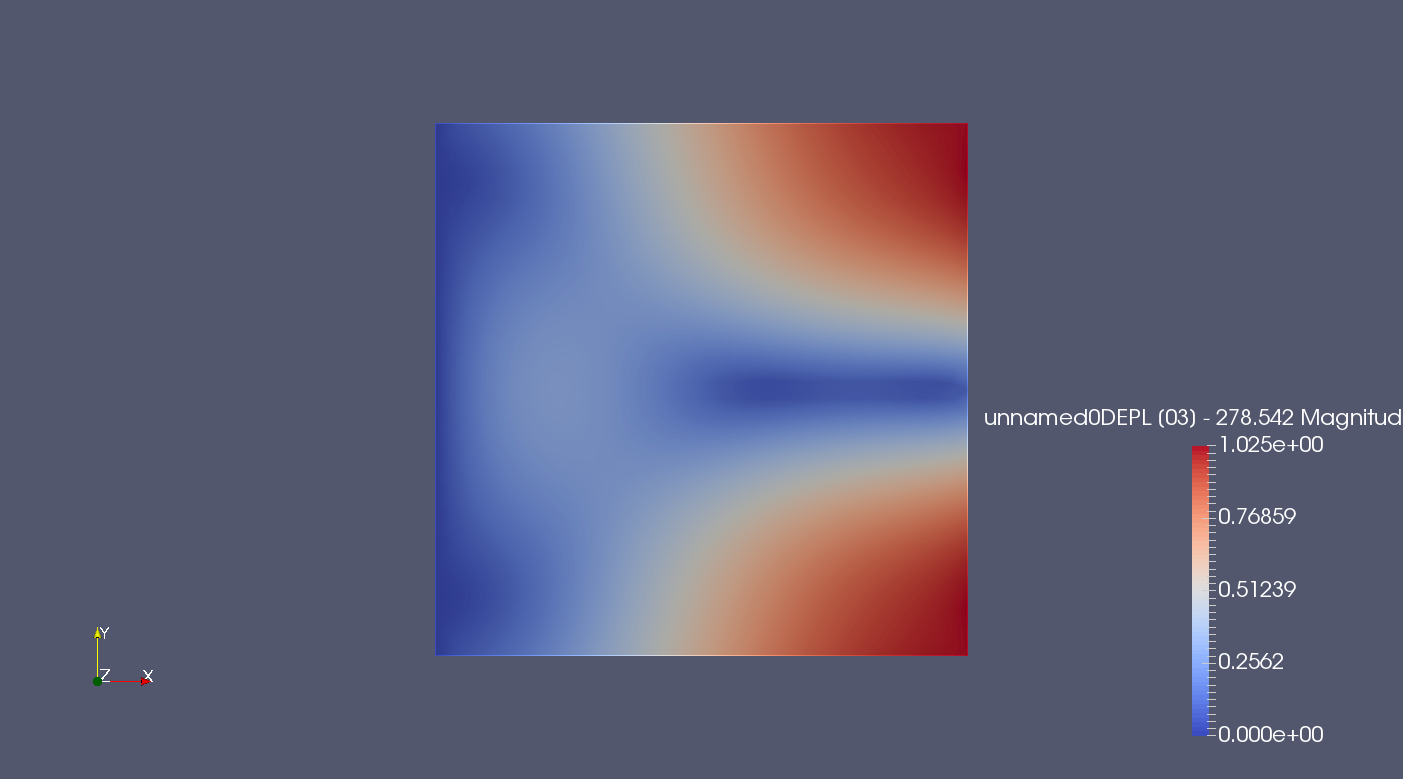
\includegraphics[width=\textwidth]{./plate_vib/278Hz.png}
  \caption{Postać modu o częstotliwości \SI{278}{\hertz}}
  \label{fig:mod1}
\end{figure}

\begin{figure}[!tbh]
  \centering
  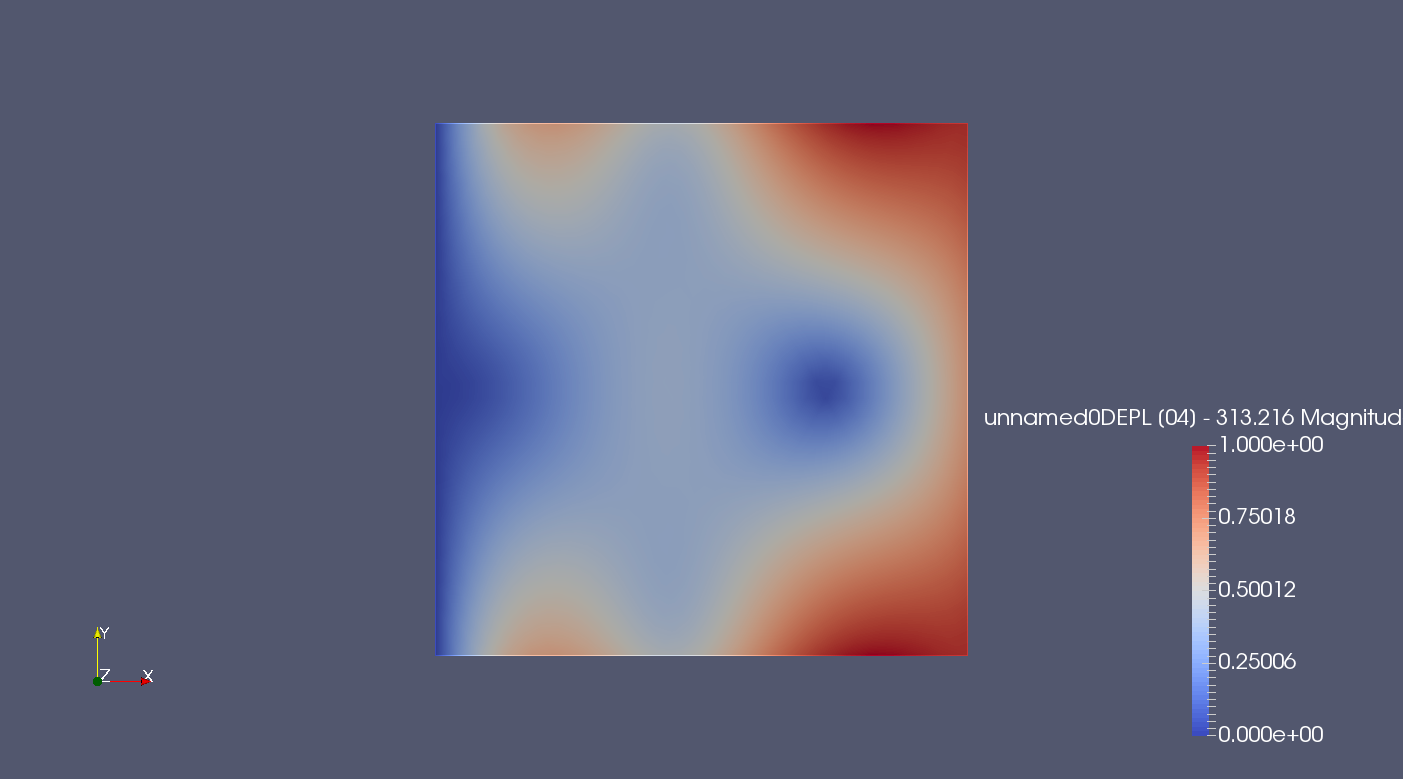
\includegraphics[width=\textwidth]{./plate_vib/313Hz.png}
  \caption{Postać modu o częstotliwości \SI{313}{\hertz}}
  \label{fig:mod2}
\end{figure}

\begin{figure}[!tbh]
  \centering
  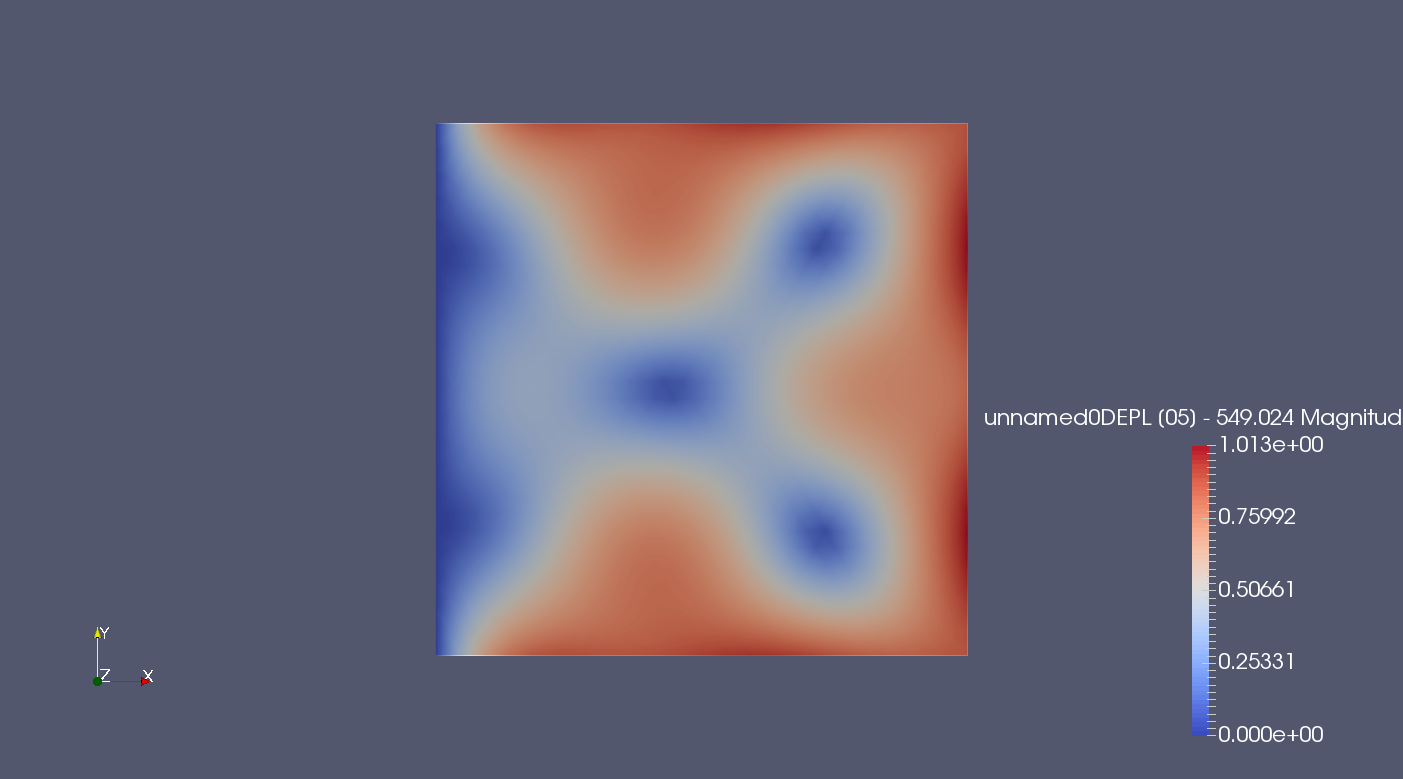
\includegraphics[width=\textwidth]{./plate_vib/549Hz.png}
  \caption{Postać modu o częstotliwości \SI{549}{\hertz}}
  \label{fig:mod3}
\end{figure}

\begin{figure}[!tbh]
  \centering
  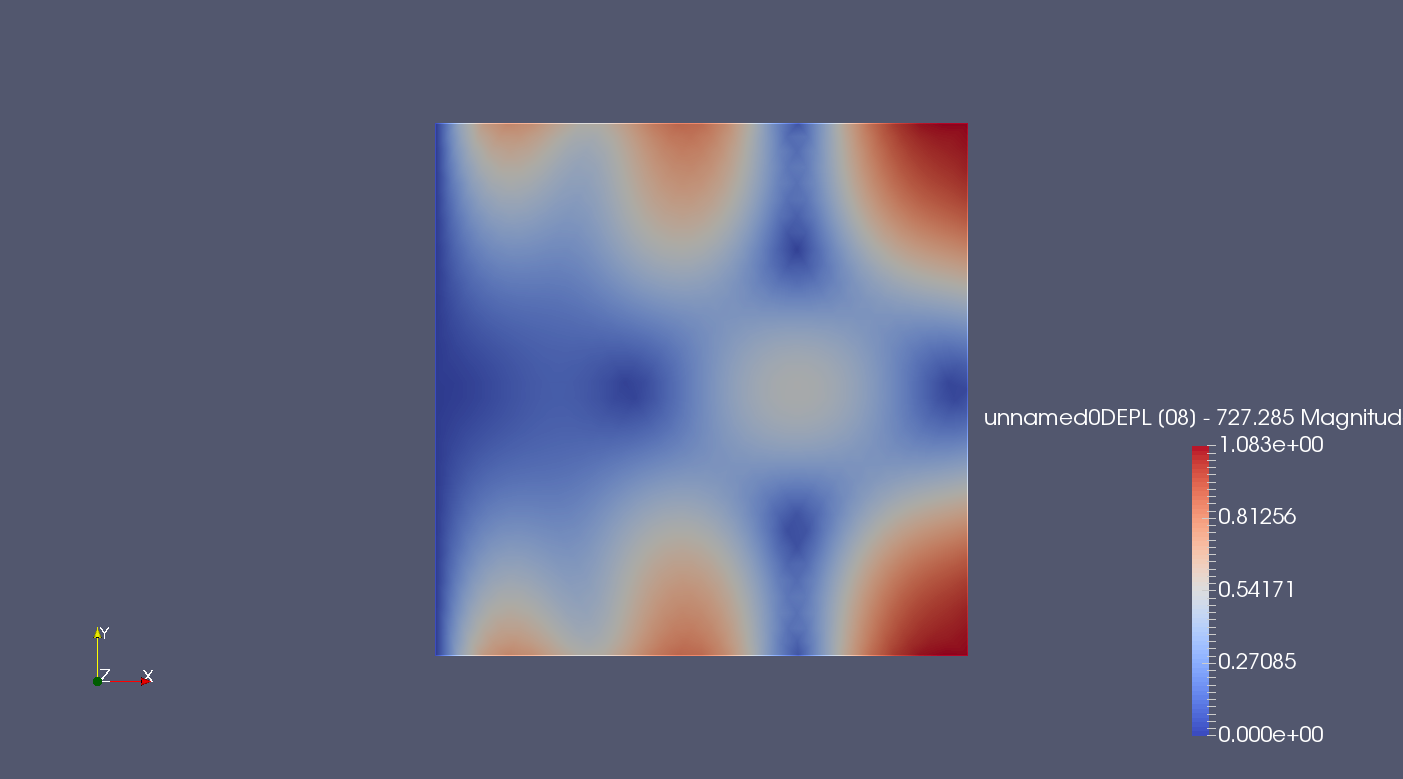
\includegraphics[width=\textwidth]{./plate_vib/727Hz.png}
  \caption{Postać modu o częstotliwości \SI{727}{\hertz}}
  \label{fig:mod4}
\end{figure}

\begin{figure}[!tbh]
  \centering
  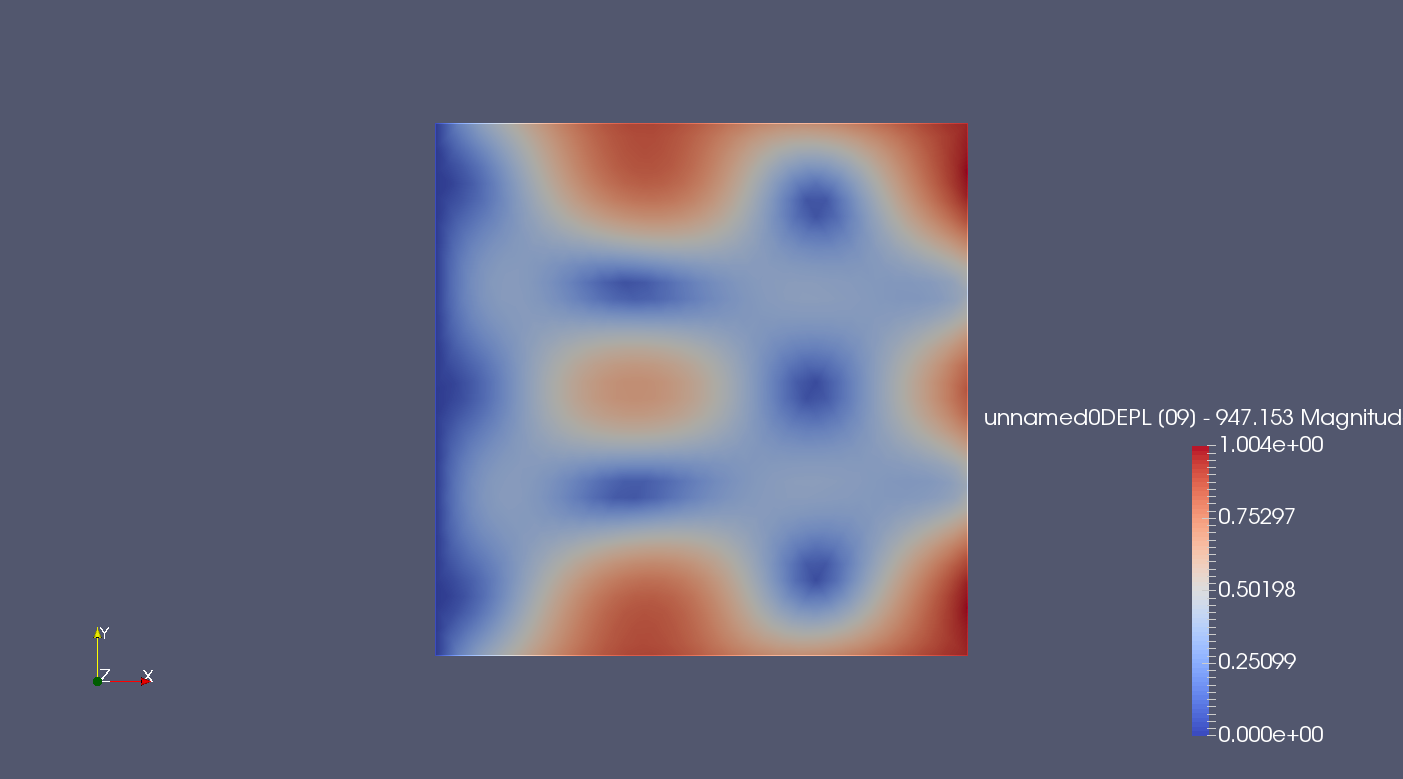
\includegraphics[width=\textwidth]{./plate_vib/947Hz.png}
  \caption{Postać modu o częstotliwości \SI{947}{\hertz}}
  \label{fig:mod5}
\end{figure}

\section{Budowa układu redukcji drgań płyty}

Na początku zaprojektowano podzespół układu do redukcji drgań płyty. Schemat
całego układu przedstawiono na rys. \ref{fig:schemat}

\begin{figure}[!tbh]
  \centering
  \import{./vecgraphics/}{PMRD_plate.pdf_tex}
  \caption{Schemat układu pomiarowego}
  \label{fig:schemat}
\end{figure}

\begin{figure}[!tbh]
  \centering
  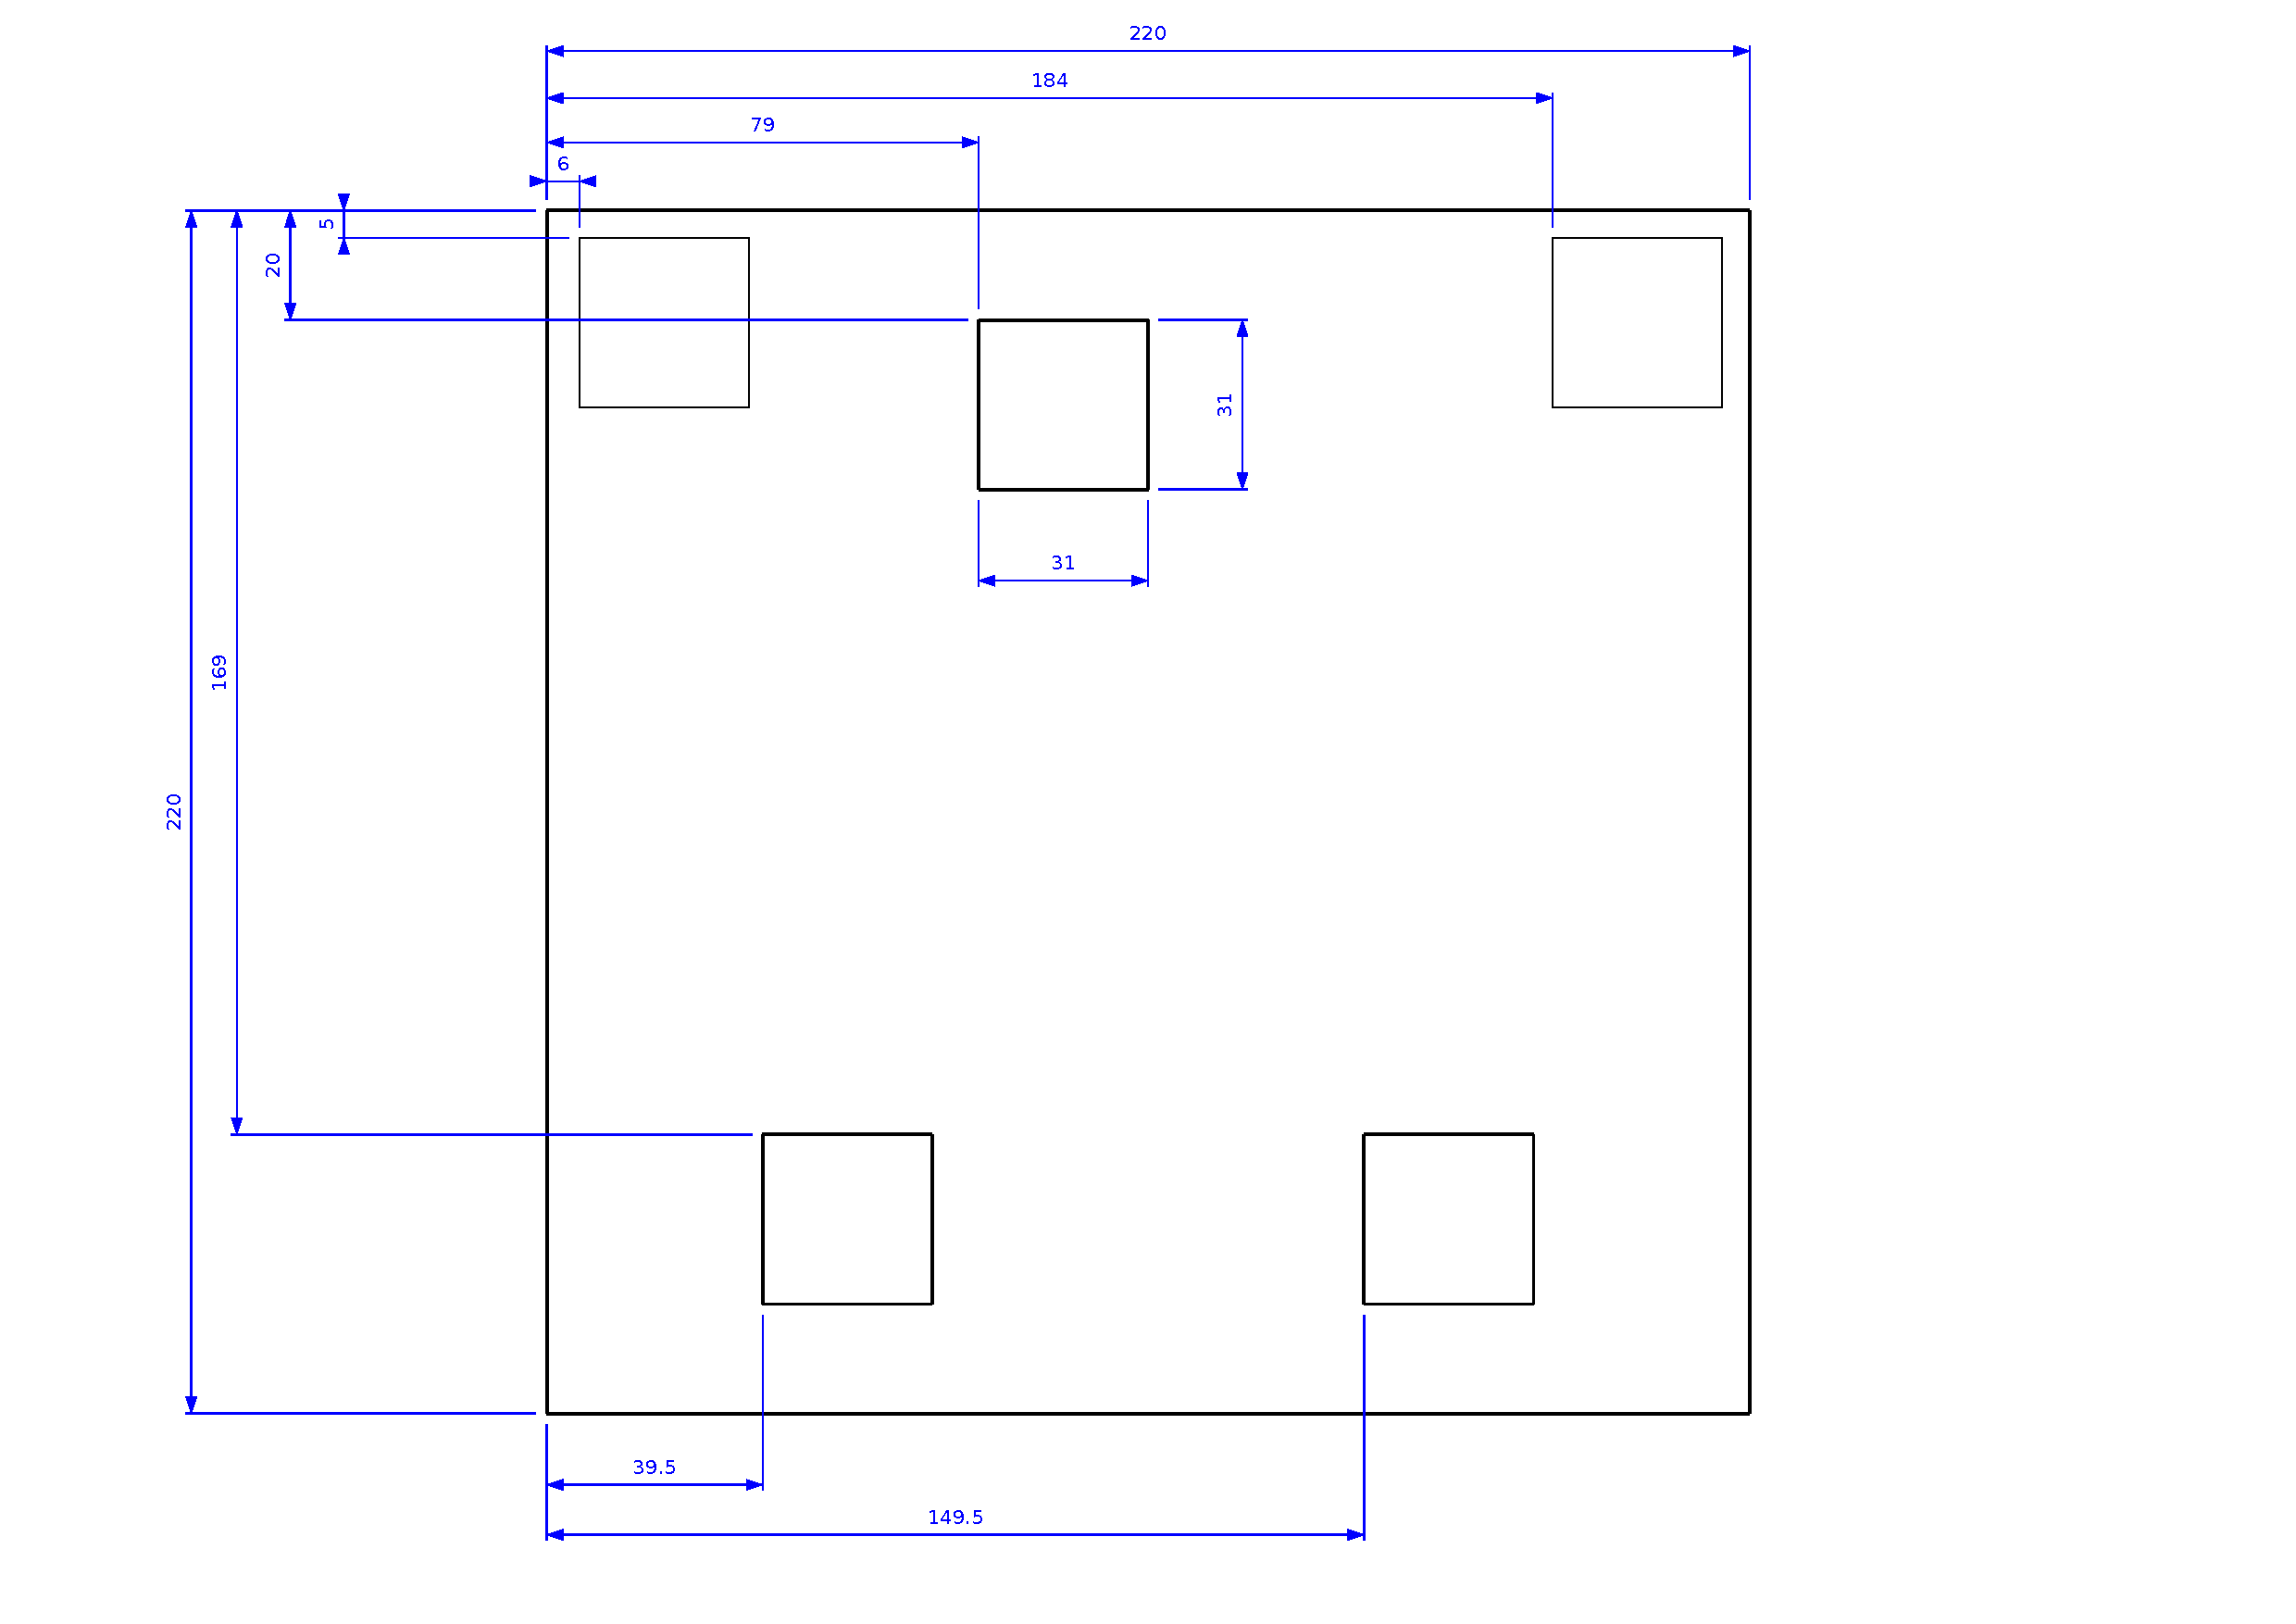
\includegraphics[width=\textwidth]{./vecgraphics/plate_dim.pdf}
  \caption{Umiejscowienie czujników}
  \label{fig:wymiary}
\end{figure}

Zbudowano część zawierającą płytę, elementy piezoelektryczne i~przewody
ostatecznie zakończone złączami BNC, które podłączono do wzmacniacza i~karty
pomiarowej.  Płyta jest aluminiowa, o wymiarach \SI{220 x 270}{\milli\meter}
(\SI{50}{\milli\meter}
przeznaczone na przymocowanie do imadła). Elementy piezoelektryczne
przymocowano do płyty wykorzystując klej dwuskładnikowy do metalu. Między
płytą, a elementami piezoelektrycznymi umieszczono miedziane płytki, na styk, o
grubości \SI{0.1}{\milli\meter} odpowiadające za przewodzenie sygnału elektrycznego między
wewnętrzną stroną piezoelektryka, a przewodem, do tej płytki przylutowanym.
Drugi przewód przylutowano do zewnętrznej strony piezoelektryka. Rozmieszczenie
elementów piezoelektrycznych (wzbudnika W, czujników $S$ i aktuatorów $A$) oraz
sposób ich przymocowania przedstawiono na rys. \ref{fig:plate1} i
\ref{fig:plate2}.

\begin{figure}[!tbh]
  \centering
  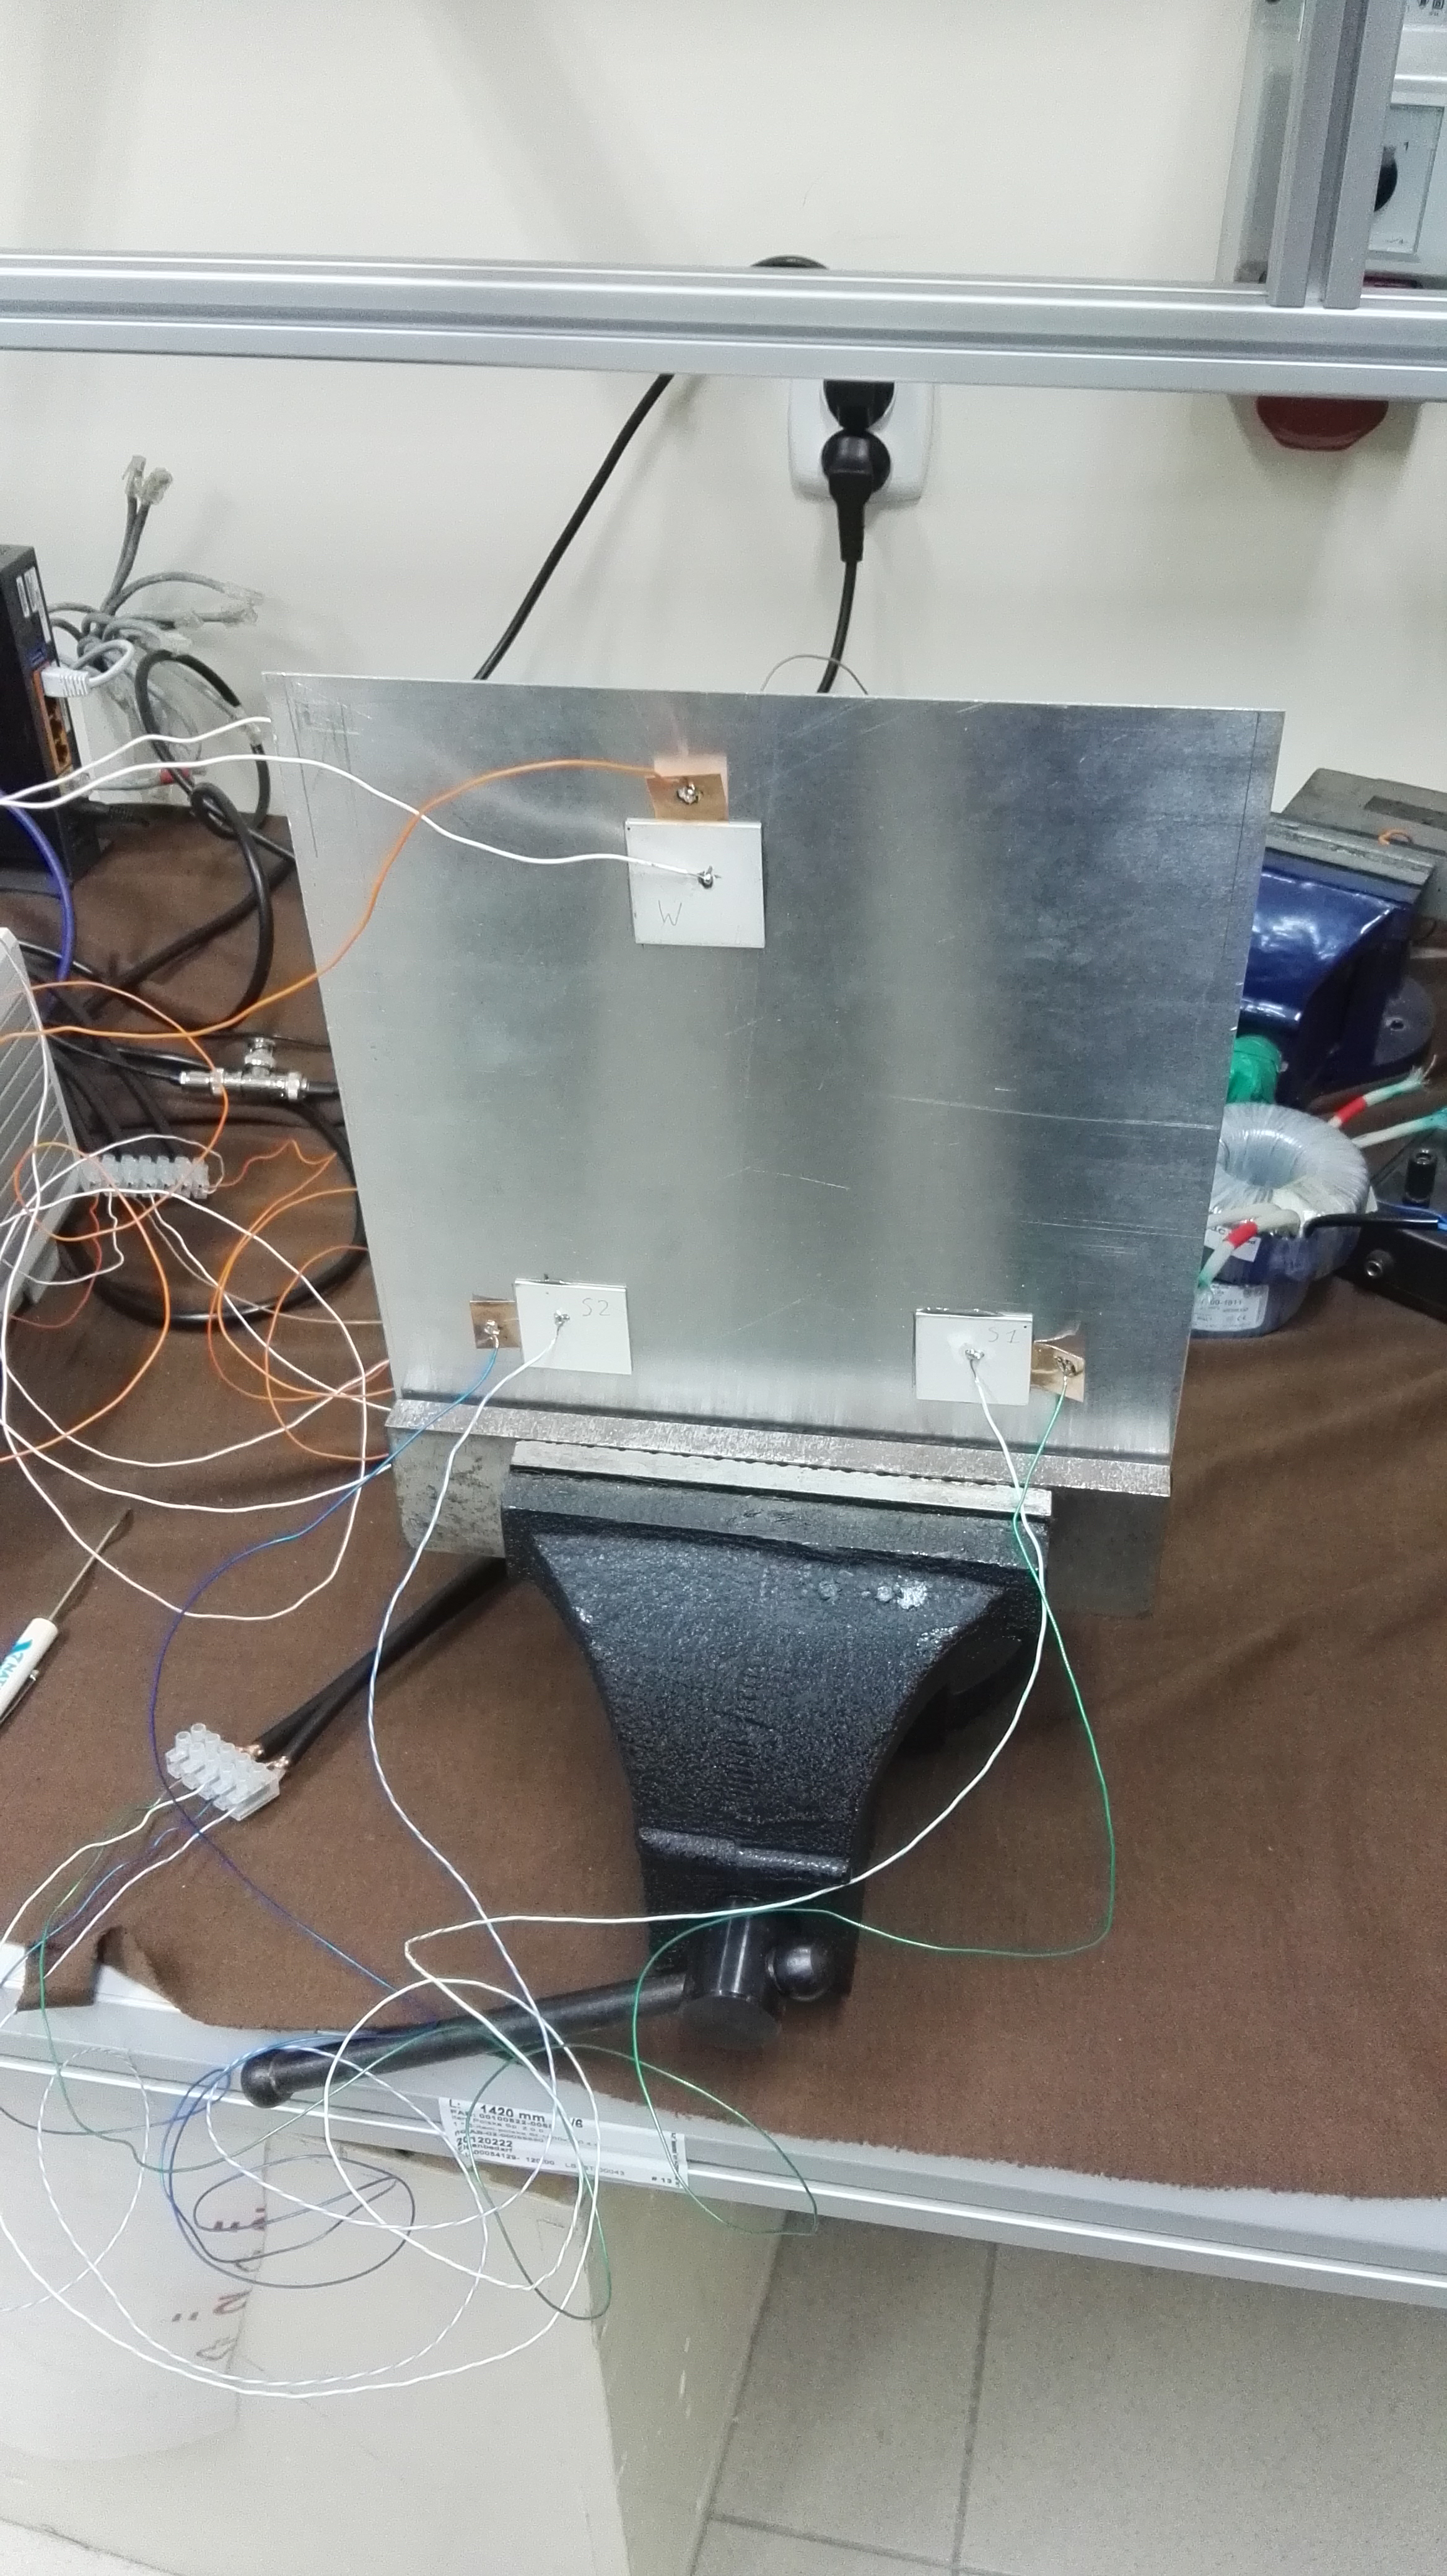
\includegraphics[width=\textwidth]{./bitgraphics/plate1.jpg}
  \caption{Widok na wzbudnik oraz czujniki zainstalowane na płycie}
  \label{fig:plate1}
\end{figure}

\begin{figure}[!tbh]
  \centering
  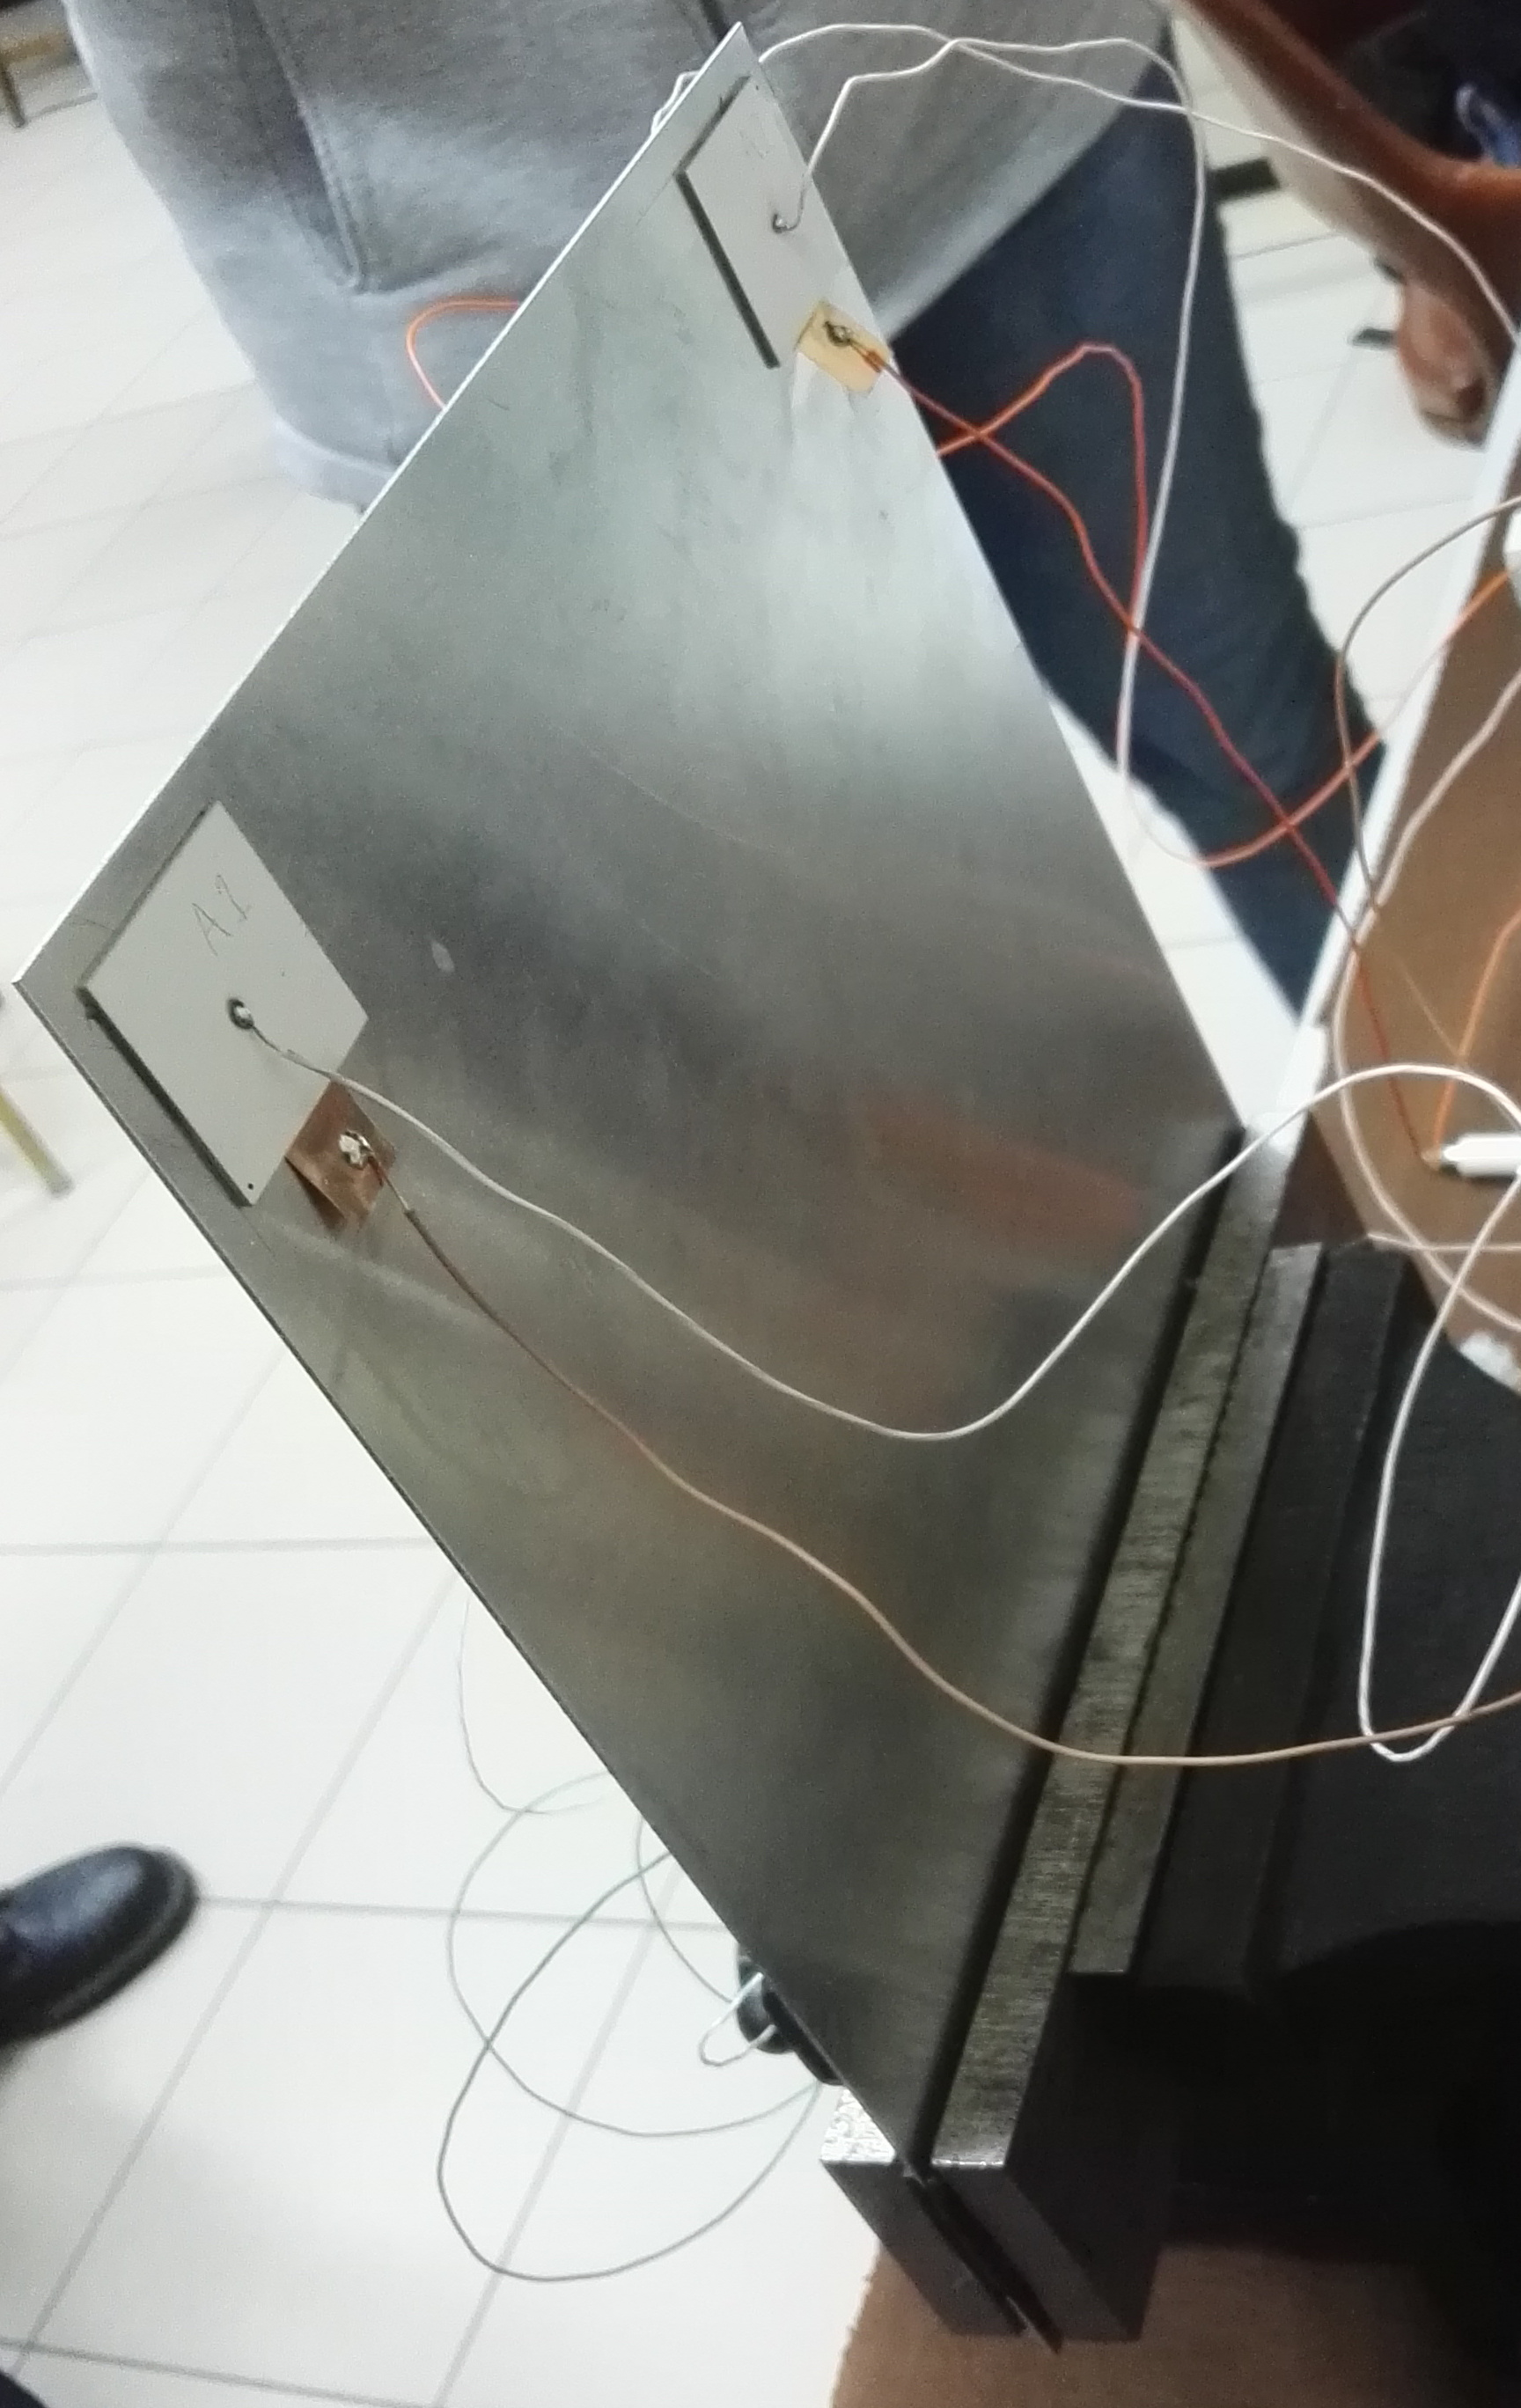
\includegraphics[width=\textwidth]{./bitgraphics/plate2.jpg}
  \caption{Widok na aktuatory zainstalowane na płycie}
  \label{fig:plate2}
\end{figure}

Drugie końce przewodów przymocowano do kostki elektrycznej, na której wyjściu
przyłączono przewody zakończone złączami BNC.

\section{Przeprowadzenie redukcji drgań płyty}

Podzespół połączono z pozostałymi elementami układu i w pierwszej kolejności
zbadano mody płyty (z elementami piezoelektrycznymi). Rezultaty przedstawiono 
w rozdziale \ref{ident}

Program wykorzystany do badania modów płyty przedstawiono na wykresach
\ref{fig:eigen_front} i \ref{fig:eigen_block}.

\begin{figure}[!tbh]
  \centering
  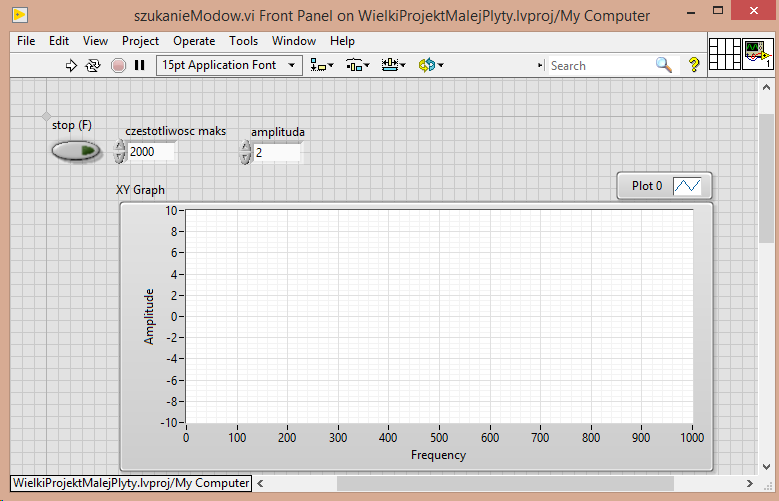
\includegraphics[width=\textwidth]{bitgraphics/panel_front_mod.png}
  \caption{Front panel programu do szukania częstotliwości własnych}
  \label{fig:eigen_front}
\end{figure}

\begin{figure}[!tbh]
  \centering
  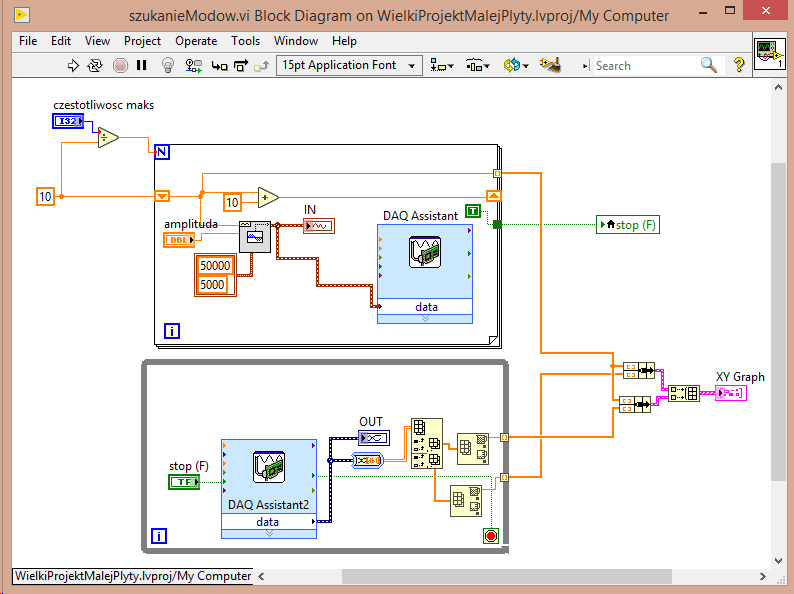
\includegraphics[width=\textwidth]{bitgraphics/panel_back_mod.png}
  \caption{Block diagram programu do szukania częstotliwości własnych}
  \label{fig:eigen_block}
\end{figure}

Program jest dwuwątkowy. W pierwszym wątku zadawane są co
\SI{100}{\milli\second} częstotliwości co \SI{10}{\hertz} od \SI{10}{\hertz} do
zadanej częstotliwości maksymalnej.  W drugim wątku zbierane są dane z
sensorów. Po zakończeniu pracy wątków dane są wyświetlane na wykresie XY Graph,
gdzie dziedziną są zadawane częstotliwości.  Dane z wykresu można eksportować
do pliku (m. in. o rozszerzeniu .txt).

W kolejnym kroku z wykorzystaniem programu napisanego w środowisku
programistycznym LabVIEW\texttrademark (rys. \ref{fig:red_front} i
\ref{fig:red_block}) dla każdej z powyżej wymienionej częstotliwości przy
stałym pobudzeniu \SI{20}{\volt} dążono do odnalezienia minimalnej amplitudy
dla czujnika $S1$, czujnika $S2$ lub sumy z tych czujników zmieniając amplitudę
oraz fazę
aktuatora $A1$, aktuatora $A2$ lub obydwu aktuatorów (każdy względem każdego, 9
konfiguracji dla każdej częstotliwości).

\begin{figure}[!tbh]
  \centering
  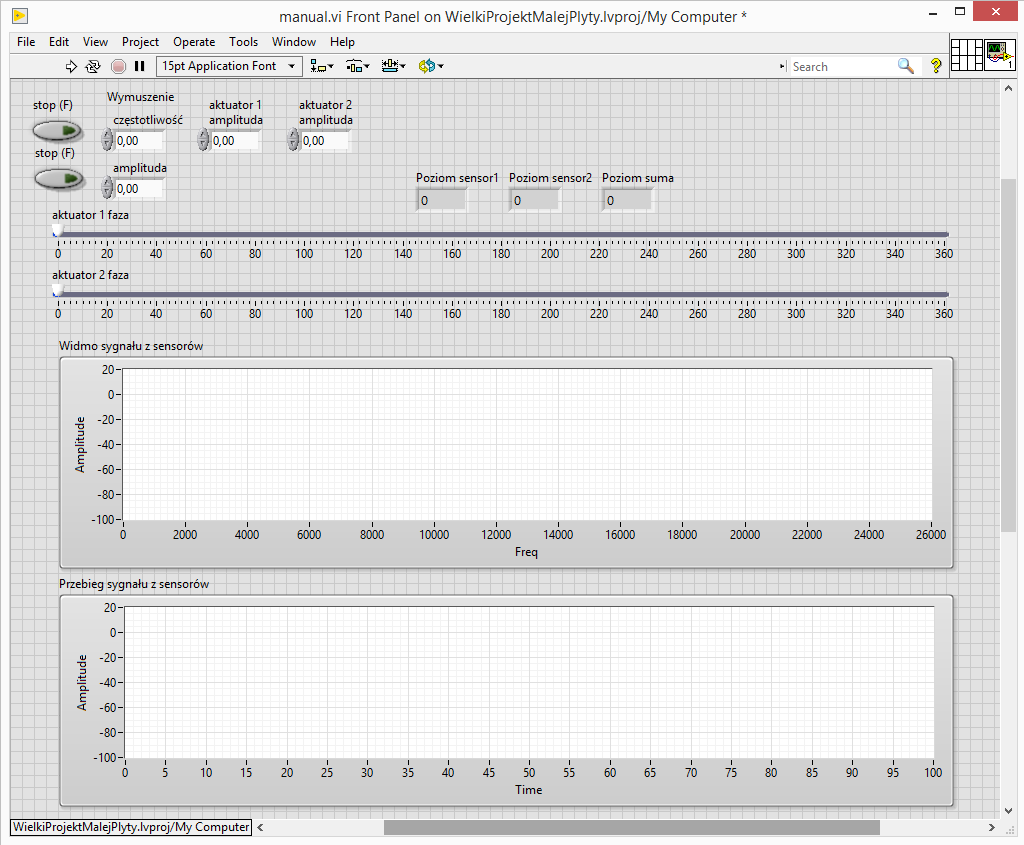
\includegraphics[width=\textwidth]{bitgraphics/panel_front_red.png}
  \caption{Front panel programu do szukania częstotliwości własnych}
  \label{fig:red_front}
\end{figure}

\begin{figure}[!tbh]
  \centering
  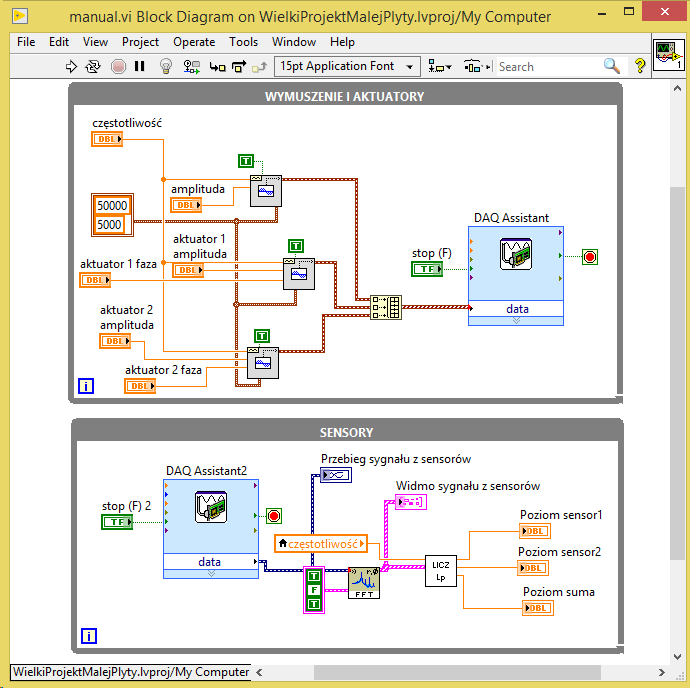
\includegraphics[width=0.9\textwidth]{bitgraphics/panel_back_red.png}
  \caption{Block diagram programu do szukania częstotliwości własnych}
  \label{fig:red_block}
\end{figure}

Program jest dwuwątkowy. W pierwszym wątku zadawane są sygnały sinusoidalne o
zadanych parametrach na piezoelektryki pełniące funkcje wymuszenia i
aktuatorów. W drugim wątku zbierane są dane z sensorów oraz przeliczane na
poziomy \si{\decibelV} dla zadanej częstotliwości. Widmo oraz przebieg sygnału
z sensorów są wyświetlane na wykresach.

\section{Wyniki}

Wyniki redukcji drgań dla kolejnych częstotliwości przedstawiono w tab.
\ref{tab:red1}--\ref{tab:red5}. Na czerwono w tablicach zaznaczono sytuacje w
których nie udało się uzyskań napięcia potrzebnego do redukcji z~powodu
niewystarczającej mocy wzmacniacza.

\begin{table}[!tbh]
  \centering
  \caption{Wyniki redukcji drgań dla modu \SI{250}{\hertz}}
  \label{tab:red1}
  \begin{tabular}{|c|c|c|c|c|c|c|}
    \cline{3-7}
    \multicolumn{2}{c|}{}&\multicolumn{2}{c|}{Aktuator}&\multicolumn{3}{c|}{Czujnik [\si{\decibelV}]}\\\cline{3-7}
    \multicolumn{2}{c|}{}&$A1$&$A2$&$S1$&$S2$&$S1+S2$\\\hline
    \multirow{2}{*}{tło}               &   $A [\si{\V}]$ & - & - & -84,0 & -90,2 & -83,3 \\\cline{2-7}
				       &$\Phi [\si{\degree}]$ & - & - & \multicolumn{3}{c}{}\\\hline
    \multirow{2}{*}{bez redukcji}      &   $A [\si{\V}]$ & - & - & -19,0 & -34,5 & -18,8 \\\cline{2-7}
				       &$\Phi [\si{\degree}]$ & - & - & \multicolumn{3}{c}{}\\\hline
    \multirow{6}{*}{$\min\{S1\}$}      &   $A [\si{\V}]$ & 29,2 & - & \textbf{-63,5} & -52,1 & -51,8 \\\cline{2-7}
				       &$\Phi [\si{\degree}]$ & 15 & - & \multicolumn{3}{c}{}\\\cline{2-7}
				       &   $A [\si{\V}]$ & - & 34,6 & \textbf{-62,8} & -42,0 & -42,0 \\\cline{2-7}
				       &$\Phi [\si{\degree}]$ & - & 23 & \multicolumn{3}{c}{}\\\cline{2-7}
				       &   $A [\si{\V}]$ & 29,2 & 0 & \textbf{-63,5} & -52,1 & -51,8 \\\cline{2-7}
				       &$\Phi [\si{\degree}]$ & 15 & 0 & \multicolumn{3}{c}{}\\\hline
    \multirow{6}{*}{$\min\{S2\}$}      &   $A [\si{\V}]$ & 27,8 & - & -36,0 & \textbf{-73,3} & -36,0\\\cline{2-7}
				       &$\Phi [\si{\degree}]$ & 10 & - & \multicolumn{3}{c}{}\\\cline{2-7}
				       &   $A [\si{\V}]$ & - & 31 & -26,8 & \textbf{-67,3} & -26,8 \\\cline{2-7}
				       &$\Phi [\si{\degree}]$ & - & 0 & \multicolumn{3}{c}{}\\\cline{2-7}
				       &   $A [\si{\V}]$ & 25,5 & 2,9 & -36,4 & \textbf{-80,1} & -36,4 \\\cline{2-7}
				       &$\Phi [\si{\degree}]$ & 6 & 69 & \multicolumn{3}{c}{}\\\hline
    \multirow{6}{*}{$\min\{S1+S2\}$}   &   $A [\si{\V}]$ & 29,2 & - & -63,5  & -52,1 & \textbf{-51,8}\\\cline{2-7}
				       &$\Phi [\si{\degree}]$ & 15 & - & \multicolumn{3}{c}{}\\\cline{2-7}
				       &   $A [\si{\V}]$ & - & 34,2 & -59,2 & -42,9 & \textbf{-42,8} \\\cline{2-7}
				       &$\Phi [\si{\degree}]$ & - & 24 & \multicolumn{3}{c}{}\\\cline{2-7}
				       &   $A [\si{\V}]$ & 29,2 & 0 & -63,5 & -52,1 & \textbf{-51,8} \\\cline{2-7}
				       &$\Phi [\si{\degree}]$ & 15 & 0 & \multicolumn{3}{c}{}\\\cline{1-4}
  \end{tabular}
\end{table}

\begin{table}[!tbh]
  \centering
  \caption{Wyniki redukcji drgań dla modu \SI{300}{\hertz}}
  \label{tab:red2}
  \begin{tabular}{|c|c|c|c|c|c|c|}
    \cline{3-7}
    \multicolumn{2}{c|}{}&\multicolumn{2}{c|}{Aktuator}&\multicolumn{3}{c|}{Czujnik [\si{\decibelV}]}\\\cline{3-7}
    \multicolumn{2}{c|}{}&$A1$&$A2$&$S1$&$S2$&$S1+S2$\\\hline
    \multirow{2}{*}{tło}               &   $A [\si{\V}]$ & - & - & -100,0 & -99,0 & -99,0 \\\cline{2-7}
				       &$\Phi [\si{\degree}]$ & - & - & \multicolumn{3}{c}{}\\\hline
    \multirow{2}{*}{bez redukcji}      &   $A [\si{\V}]$ & - & - & -19,9 & -40,0 & -19,9 \\\cline{2-7}
				       &$\Phi [\si{\degree}]$ & - & - & \multicolumn{3}{c}{}\\\hline
    \multirow{6}{*}{$\min\{S1\}$}      &   $A [\si{\V}]$ & \textcolor{red}{51} & - & \textbf{-29,7} & -45,0 & -21,7\\\cline{2-7}
				       &$\Phi [\si{\degree}]$ & 292 & - & \multicolumn{3}{c}{}\\\cline{2-7}
				       &   $A [\si{\V}]$ & - & \textcolor{red}{40} & \textbf{-22,0} & -43,6 & -22,0 \\\cline{2-7}
				       &$\Phi [\si{\degree}]$ & - & 180 & \multicolumn{3}{c}{}\\\cline{2-7}
				       &   $A [\si{\V}]$ & \textcolor{red}{51} & 0 & \textbf{-29,7} & -45,0 & -22,0 \\\cline{2-7}
				       &$\Phi [\si{\degree}]$ & 292 & 0 & \multicolumn{3}{c}{}\\\hline
    \multirow{6}{*}{$\min\{S2\}$}      &   $A [\si{\V}]$ & \textcolor{red}{51} & - & -29,7 & \textbf{-45,0} & -21,7 \\\cline{2-7}
				       &$\Phi [\si{\degree}]$ & 292 & - & \multicolumn{3}{c}{}\\\cline{2-7}
				       &   $A [\si{\V}]$ & - & \textcolor{red}{40} & -21,5 & \textbf{-44,6} & -21,4 \\\cline{2-7}
				       &$\Phi [\si{\degree}]$ & - & 210 & \multicolumn{3}{c}{}\\\cline{2-7}
				       &   $A [\si{\V}]$ & \textcolor{red}{51} & \textcolor{red}{40} & -23,7 & \textbf{-59,5} & -13,7\\\cline{2-7}
				       &$\Phi [\si{\degree}]$ & 291 & 211 & \multicolumn{3}{c}{}\\\hline
    \multirow{6}{*}{$\min\{S1+S2\}$}   &   $A [\si{\V}]$ & \textcolor{red}{51} & - & -29,7 & -45,0 & \textbf{-21,7}\\\cline{2-7}
				       &$\Phi [\si{\degree}]$ & 292 & - & \multicolumn{3}{c}{}\\\cline{2-7}
				       &   $A [\si{\V}]$ & - & \textcolor{red}{40} & -22,0 & -43,6 & \textbf{-22,0} \\\cline{2-7}
				       &$\Phi [\si{\degree}]$ & - & 180 & \multicolumn{3}{c}{}\\\cline{2-7}
				       &   $A [\si{\V}]$ & \textcolor{red}{51} & \textcolor{red}{40} & -24,5 & -51,3 & \textbf{-24,5} \\\cline{2-7}
				       &$\Phi [\si{\degree}]$ & 294 & 180 & \multicolumn{3}{c}{}\\\cline{1-4}
  \end{tabular}
\end{table}

\begin{table}[!tbh]
  \centering
  \caption{Wyniki redukcji drgań dla modu \SI{570}{\hertz}}
  \label{tab:red3}
  \begin{tabular}{|c|c|c|c|c|c|c|}
    \cline{3-7}
    \multicolumn{2}{c|}{}&\multicolumn{2}{c|}{Aktuator}&\multicolumn{3}{c|}{Czujnik [\si{\decibelV}]}\\\cline{3-7}
    \multicolumn{2}{c|}{}&$A1$&$A2$&$S1$&$S2$&$S1+S2$\\\hline
    \multirow{2}{*}{tło}               &   $A [\si{\V}]$ & - & - & -82,7 & -97,5 & -82,8 \\\cline{2-7}
				       &$\Phi [\si{\degree}]$ & - & - & \multicolumn{3}{c}{}\\\hline
    \multirow{2}{*}{bez redukcji}      &   $A [\si{\V}]$ & - & - & -10,2 & -31,5 & -10,2 \\\cline{2-7}
				       &$\Phi [\si{\degree}]$ & - & - & \multicolumn{3}{c}{}\\\hline
    \multirow{6}{*}{$\min\{S1\}$}      &   $A [\si{\V}]$ & 44 & - & \textbf{-54,5} & -38,0 & -37,9 \\\cline{2-7}
				       &$\Phi [\si{\degree}]$ & 26 & - & \multicolumn{3}{c}{}\\\cline{2-7}
				       &   $A [\si{\V}]$ & - & 35,7 & \textbf{-40,5} & -33,9 & -33 \\\cline{2-7}
				       &$\Phi [\si{\degree}]$ & - & 355 & \multicolumn{3}{c}{}\\\cline{2-7}
				       &   $A [\si{\V}]$ & 1,9 & 35,7 & \textbf{-65,2} & -34,0 & -34,0\\\cline{2-7}
				       &$\Phi [\si{\degree}]$ & 108 & 355 & \multicolumn{3}{c}{}\\\hline
    \multirow{6}{*}{$\min\{S2\}$}      &   $A [\si{\V}]$ & 44 & - & -17,3 & \textbf{-55,6} & -17,3 \\\cline{2-7}
				       &$\Phi [\si{\degree}]$ & 0 & - & \multicolumn{3}{c}{}\\\cline{2-7}
				       &   $A [\si{\V}]$ & - & \textcolor{red}{40} & -11,7 & \textbf{-44,1} & -11,7 \\\cline{2-7}
				       &$\Phi [\si{\degree}]$ & - & 42 & \multicolumn{3}{c}{}\\\cline{2-7}
				       &   $A [\si{\V}]$ & 44 & 3 & -15,8 & \textbf{-81,3} & -15,8 \\\cline{2-7}
				       &$\Phi [\si{\degree}]$ & 0 & 238 & \multicolumn{3}{c}{}\\\hline
    \multirow{6}{*}{$\min\{S1+S2\}$}   &   $A [\si{\V}]$ & 44 & - & -54,5 & -38,0 & \textbf{-37,9}\\\cline{2-7}
				       &$\Phi [\si{\degree}]$ & 26 & - & \multicolumn{3}{c}{}\\\cline{2-7}
				       &   $A [\si{\V}]$ & - & 35,7 & -40,5 & -33,9 & \textbf{-33} \\\cline{2-7}
				       &$\Phi [\si{\degree}]$ & - & 355 & \multicolumn{3}{c}{}\\\cline{2-7}
				       &   $A [\si{\V}]$ & 44 & 0 & -54,5 & -38,0 & \textbf{-37,9} \\\cline{2-7}
				       &$\Phi [\si{\degree}]$ & 26 & 0 & \multicolumn{3}{c}{}\\\cline{1-4}
  \end{tabular}
\end{table}

\begin{table}[!tbh]
  \centering
  \caption{Wyniki redukcji drgań dla modu \SI{710}{\hertz}}
  \label{tab:red4}
  \begin{tabular}{|c|c|c|c|c|c|c|}
    \cline{3-7}
    \multicolumn{2}{c|}{}&\multicolumn{2}{c|}{Aktuator}&\multicolumn{3}{c|}{Czujnik [\si{\decibelV}]}\\\cline{3-7}
    \multicolumn{2}{c|}{}&$A1$&$A2$&$S1$&$S2$&$S1+S2$\\\hline
    \multirow{2}{*}{tło}               &   $A [\si{\V}]$ & - & - & -80,0 & -94,1 & -80,0 \\\cline{2-7}
				       &$\Phi [\si{\degree}]$ & - & - & \multicolumn{3}{c}{}\\\hline
    \multirow{2}{*}{bez redukcji}      &   $A [\si{\V}]$ & - & - & -9,5 & -29,6 & -9,4 \\\cline{2-7}
				       &$\Phi [\si{\degree}]$ & - & - & \multicolumn{3}{c}{}\\\hline
    \multirow{6}{*}{$\min\{S1\}$}      &   $A [\si{\V}]$ & 37,9 & - & \textbf{-56,3} & -52,5 & -51,0 \\\cline{2-7}
				       &$\Phi [\si{\degree}]$ & 238 & - & \multicolumn{3}{c}{}\\\cline{2-7}
				       &   $A [\si{\V}]$ & - & \textcolor{red}{40} & \textbf{-17,3} & -32,0 & -17,1 \\\cline{2-7}
				       &$\Phi [\si{\degree}]$ & - & 248 & \multicolumn{3}{c}{}\\\cline{2-7}
				       &   $A [\si{\V}]$ & 37,5 & 0,4 & \textbf{-65,4} & -48,8 & -48,8 \\\cline{2-7}
				       &$\Phi [\si{\degree}]$ & 238 & 326 & \multicolumn{3}{c}{}\\\hline
    \multirow{6}{*}{$\min\{S2\}$}      &   $A [\si{\V}]$ & 35,5 & - & -32,1 & \textbf{-82,5} & -32,1 \\\cline{2-7}
				       &$\Phi [\si{\degree}]$ & 236 & - & \multicolumn{3}{c}{}\\\cline{2-7}
				       &   $A [\si{\V}]$ & - & \textcolor{red}{39} & -16,4 & \textbf{-32,6} & -16,3 \\\cline{2-7}
				       &$\Phi [\si{\degree}]$ & - & 257 & \multicolumn{3}{c}{}\\\cline{2-7}
				       &   $A [\si{\V}]$ & 35,5 & 0 & -32,1 & \textbf{-82,5} & -32,1\\\cline{2-7}
				       &$\Phi [\si{\degree}]$ & 236 & 0 & \multicolumn{3}{c}{}\\\hline
    \multirow{6}{*}{$\min\{S1+S2\}$}   &   $A [\si{\V}]$ & 37,9 & - & -56,3 & -52,5 & \textbf{-51,0}\\\cline{2-7}
				       &$\Phi [\si{\degree}]$ & 238 & - & \multicolumn{3}{c}{}\\\cline{2-7}
				       &   $A [\si{\V}]$ & - & \textcolor{red}{40} & -17,3 & -32,0 & \textbf{-17,1} \\\cline{2-7}
				       &$\Phi [\si{\degree}]$ & - & 248 & \multicolumn{3}{c}{}\\\cline{2-7}
				       &   $A [\si{\V}]$ & 37,9 & 0,4 & -61,7 & -52,9 & \textbf{-52,3} \\\cline{2-7}
				       &$\Phi [\si{\degree}]$ & 238 & 0 & \multicolumn{3}{c}{}\\\cline{1-4}
  \end{tabular}
\end{table}

\begin{table}[!tbh]
  \centering
  \caption{Wyniki redukcji drgań dla modu \SI{920}{\hertz}}
  \label{tab:red5}
  \begin{tabular}{|c|c|c|c|c|c|c|}
    \cline{3-7}
    \multicolumn{2}{c|}{}&\multicolumn{2}{c|}{Aktuator}&\multicolumn{3}{c|}{Czujnik [\si{\decibelV}]}\\\cline{3-7}
    \multicolumn{2}{c|}{}&$A1$&$A2$&$S1$&$S2$&$S1+S2$\\\hline
    \multirow{2}{*}{tło}               &   $A [\si{\V}]$ & - & - & -89,4 & -100,0 & -89,5 \\\cline{2-7}
				       &$\Phi [\si{\degree}]$ & - & - & \multicolumn{3}{c}{}\\\hline
    \multirow{2}{*}{bez redukcji}      &   $A [\si{\V}]$ & - & - & -7,5 & -24,3 & -7,4 \\\cline{2-7}
				       &$\Phi [\si{\degree}]$ & - & - & \multicolumn{3}{c}{}\\\hline
    \multirow{6}{*}{$\min\{S1\}$}      &   $A [\si{\V}]$ & 21,4 & - & \textbf{-58,3} & -31,2 & -31,2 \\\cline{2-7}
				       &$\Phi [\si{\degree}]$ & 172 & - & \multicolumn{3}{c}{}\\\cline{2-7}
				       &   $A [\si{\V}]$ & - & 36,6 & \textbf{-62,0} & -29,3 & -29,3 \\\cline{2-7}
				       &$\Phi [\si{\degree}]$ & - & 356 & \multicolumn{3}{c}{}\\\cline{2-7}
				       &   $A [\si{\V}]$ & 1,7 & 36,6 & \textbf{-62,1} & -29,4 & -29,4 \\\cline{2-7}
				       &$\Phi [\si{\degree}]$ & 85 & 0 & \multicolumn{3}{c}{}\\\hline
    \multirow{6}{*}{$\min\{S2\}$}      &   $A [\si{\V}]$ & 35,8 & - & -9,8 & \textbf{-74,9} & -9,8\\\cline{2-7}
				       &$\Phi [\si{\degree}]$ & 184 & - & \multicolumn{3}{c}{}\\\cline{2-7}
				       &   $A [\si{\V}]$ & - & \textcolor{red}{40} & -12,4 & \textbf{-35,6} & -12,4 \\\cline{2-7}
				       &$\Phi [\si{\degree}]$ & - & 26 & \multicolumn{3}{c}{}\\\cline{2-7}
				       &   $A [\si{\V}]$ & 35,7 & 0,4 & -9,7 & \textbf{-77,4} & -9,7\\\cline{2-7}
				       &$\Phi [\si{\degree}]$ & 184 & 332 & \multicolumn{3}{c}{}\\\hline
    \multirow{6}{*}{$\min\{S1+S2\}$}   &   $A [\si{\V}]$ & 21,4 & - & -58,3 & -31,2 & \textbf{-31,2} \\\cline{2-7}
				       &$\Phi [\si{\degree}]$ & 172 & - & \multicolumn{3}{c}{}\\\cline{2-7}
				       &   $A [\si{\V}]$ & - & 36,6 & -62,0 & -29,3 & \textbf{-29,3} \\\cline{2-7}
				       &$\Phi [\si{\degree}]$ & - & 356 & \multicolumn{3}{c}{}\\\cline{2-7}
				       &   $A [\si{\V}]$ & 21,4 & 0 & -58,3 & -31,2 & \textbf{-31,2} \\\cline{2-7}
				       &$\Phi [\si{\degree}]$ & 172 & 0 & \multicolumn{3}{c}{}\\\cline{1-4}
  \end{tabular}
\end{table}

\section{Analiza wyników}

\begin{table}[!tbh]
  \centering
  \caption{Wartości redukcji drgań dla badanych częstotliwości}
  \begin{tabular}{|c|c|c|c|c|c|c|}
    \cline{3-7}
    \multicolumn{2}{c|}{} & \multicolumn{5}{c|}{Częstotliwość [\si{\hertz}]} \\\cline{3-7}
	\multicolumn{2}{c|}{}			& 250 & 300 & 570 & 710 & 920 \\\cline{2-7}
	\multicolumn{1}{c|}{} & Aktuator & \multicolumn{5}{c|}{Redukcja [\si{\decibelV}]} \\\hline
    \multirow{3}{*}{$\min\{S1\}$}      & $A1$      & 44,5 & 9,8 & 44,3 & 46,8 & 50,8 \\\cline{2-7}
				       & $A2$      & 43,8 & 2,1 & 30,3 & 7,8 & 54,5 \\\cline{2-7}
				       & $A1 + A2$ & 44,5 & 9,8 & 55,0 & 55,9 & 54,6 \\\hline
    \multirow{3}{*}{$\min\{S2\}$}      & $A1$      & 38,8 & 5,0 & 24,1 & 52,9 & 50,6 \\\cline{2-7}
				       & $A2$      & 32,8 & 4,6 & 12,6 & 3,0 & 11,3 \\\cline{2-7}
				       & $A1 + A2$ & 45,6 & 19,5 & 49,8 & 52,9 & 53,1 \\\hline
    \multirow{3}{*}{$\min\{S1 + S2\}$} & $A1$      & 33,0 & 2,6 & 27,7 & 41,6 & 23,8 \\\cline{2-7}
				       & $A2$      & 24,0 & 2,9 & 22,8 & 7,7 & 21,9 \\\cline{2-7}
				       & $A1 + A2$ & 33,0 & 5,4 & 27,7 & 42,9 & 23,8 \\\hline
  \end{tabular}
  \label{tab:redukcja}
\end{table}

Dla częstotliwości \SI{250}{\hertz} skutecznie całkowicie wytłumiono drgania
względem czujnika $S2$ z wykorzystaniem dwóch aktuatorów. Dobry efekt też dała
modulacja jedynie aktuatorem $A1$. Względem pojedynczego czujnika
maksymalnie udało się stłumić amplitudę drgań o ok \SI{45}{\decibelV}, względem
sumy czujników o ok \SI{33}{\decibelV}.

Dla częstotliwości \SI{300}{\hertz} nie udało się uzyskać całkowitego
wytłumienia. Za niska była maksymalna wartość amplitudy, jaką można było zadać
z~aktuatorów.  Dla czujnika $S1$ maksymalnie udało się stłumić o ok.
\SI{10}{\decibelV}, dla $S2$ o ok. \SI{20}{\decibelV}, a dla sumy
\SI{5}{\decibelV}.

Dla częstotliwości \SI{570}{\hertz} podobnie jak dla \SI{250}{\hertz}
skutecznie całkowicie wytłumiono drgania względem czujnika $S2$ z wykorzystaniem
dwóch aktuatorów. Dla czujnika $S1$ maksymalnie udało się stłumić o ok.
\SI{55}{\decibelV}, dla $S2$ o ok. \SI{50}{\decibelV}, a dla sumy
\SI{28}{\decibelV}.

Dla częstotliwości \SI{710}{\hertz} w większości przypadków za niska była
maksymalna wartość amplitudy, jaką można było zadać z aktuatora $A2$.
Podobnie jak dla 250 oraz \SI{570}{\hertz} skutecznie całkowicie wytłumiono
drgania względem czujnika $S2$ z wykorzystaniem dwóch aktuatorów, a nawet samego
aktuatora $A1$. Dla czujnika $S1$ maksymalnie udało się stłumić
amplitudę drgań o ok. \SI{55}{\decibelV}, dla $S2$ o ok.
\SI{50}{\decibelV}, a dla sumy \SI{43}{\decibelV}.

Dla częstotliwości \SI{920}{\hertz} w jednym przypadku  za niska była
maksymalna wartość amplitudy, jaką można było zadać z aktuatora $A2$. Dla
czujnika $S1$ maksymalnie udało się stłumić amplitudę drgań o ok.
\SI{55}{\decibelV}, dla $S2$ o ok.  \SI{53}{\decibelV}, a dla sumy
\SI{25}{\decibelV}.

\section{Wnioski}

Przeprowadzono redukcję drgań płyty dla pięciu częstotliwości. Nie dla każdej
częstotliwości możliwe było całkowite wytłumienie drgań względem wybranych
czujników. Możliwość zadawania drgań dwoma aktuatorami pozwoliła w wielu
przypadkach (dla \SI{250}{\hertz} względem $S2$, \SI{300}{\hertz} względem $S2$
i $S2+S1$, dla \SI{570}{\hertz} względem $S1$ i $S2$, dla \SI{710}{\hertz}
względem $S1$ i $S1+S2$, dla \SI{900}{\hertz} względem $S1$ i $S2$) na większą
redukcję drgań niż z wykorzystaniem jednego aktuatora. Większą redukcję drgań
można było uzyskać dla redukcji lokalnej niż globalnej.


Według ustalonej miary porównawczej częstotliwości największe wahania występują
dla częstotliwości odniesienia \SI{250}{\hertz}. W pozostałych przypadkach nie
przekraczały one \SI{10}{\percent}. Wykorzystano dwie metody estymowania
częstotliwości modu: symulacja MES oraz obliczenia teoretyczne. W oparciu o
wyniki dla ustalonej miary porównawczej można stwierdzić, że symulacja MES
pozwoliła na dokładniejszą estymację dla wyższych modów (powyżej
\SI{300}{\hertz}), natomiast obliczenia teoretyczne dały lepsze wyniki dla
niższych modów. Po zaobserwowanych różnicach można jednak określić, że
symulacja MES dała wyniki estymowania modów bardziej zbliżone do zmierzonych
częstotliwości z pomiarów.  Różnice w częstotliwościach wynikały między innymi
z:
\begin{itemize}
  \item dodatkowych elementów znajdujących się na płycie zwiększających jej masę i nie
    uwzględnionych w estymacjach (elementy piezoelektryczne, płytki miedziane,
    luty, przewody), 
  \item błędu wykonania płyty (różnice w wymiarach rzeczywistych, a przyjętych),
    nieidealnego utwierdzenia,
  \item błędu pomiaru,
  \item niedokładnego przymocowania elementów piezoelektrycznych wykorzystanych
    do pomiarów.
\end{itemize}%
Niższa amplituda drgań dla czujnika $S2$ mogła wynikać z nieodpowiedniego
przyklejenia czujnika do płyty (za mało kleju, nieodpowiednio rozprowadzony, za
mała powierzchnia styku z płytą) lub z uszkodzenia elementu piezoelektrycznego
(nie został on sprawdzony przed zamontowaniem). Nieznane są inne możliwe
przyczyny, jednak nie wykluczone jest ich występowanie.

\printbibliography[title=Bibliografia]

\end{document}
